\documentclass[11pt]{article}

\usepackage{fancyhdr}
\usepackage[margin=1in]{geometry}
\usepackage{xcolor,colortbl}
\usepackage[labelfont=bf,font=small]{caption}


\usepackage[T1]{fontenc}

\usepackage{enumitem}
\usepackage{todonotes}
\usepackage{titlesec}
\usepackage{tabularx}
\usepackage{parskip}
\usepackage{hyperref}
\usepackage{wrapfig}
\titlespacing\section{0pt}{0pt plus 4pt minus 2pt}{0pt plus 2pt minus 2pt}
\titlespacing\subsection{0pt}{12pt plus 4pt minus 2pt}{0pt plus 2pt minus 2pt}
\titlespacing\subsubsection{0pt}{12pt plus 4pt minus 2pt}{0pt plus 2pt minus 2pt}

\definecolor{Gray}{gray}{0.85}
\pagestyle{fancy}
\rfoot{\thepage}
\lfoot{\textbf{Research Statement} | D.A. Szafir}
\cfoot{}
\renewcommand{\headrulewidth}{0pt}
\renewcommand{\footrulewidth}{0.5pt}

%opening


\begin{document}
\setlength{\belowcaptionskip}{-10pt}
%\maketitle

\thispagestyle{fancy}

\textbf{\Large Research Statement}
{\hspace{220pt}\emph{Danielle Albers Szafir} \vspace{3pt}}
\hrule
%\\
%	{ 
%	\begin{tabularx}{\textwidth}{X X}
%		Assistant Professor & 315 UCB\\ 
%		Department of Information Science & University of Colorado Boulder \\ 
%		College of Media, Communication, \& Information &  Boulder, CO, 80309\\
%		University of Colorado Boulder & danielle.szafir@colorado.edu | 303.492.8532 
%	\end{tabularx}}}
%\hrule

%My research fuses methods from computer science, vision science, and cognitive science to model visual perception in order to develop novel visualization systems which support accurate analysis of complex data at unprecedented scales. These systems provide new analytics solutions in domains ranging from biology to the humanities. Through this work, I expand knowledge of visualization design by considering how the ubiquity and scales of data analysis fundamentally shift the demands placed on analytics tools.  %\vspace{-2pt}

Visualizations have traditionally relied on perceptual models from psychology to guide designs that communicate relationships in data.  However, these models ignore the complexities arising in real-world analytics applications, such as imperfect displays and crowded data distributions. These oversimplifications can cause people to misinterpret their data, leading to scalability limitations, flawed understandings, and erroneous conclusions. Further, advances in technologies such as statistical analytics techniques and novel display technologies offer new opportunities 
%for effective and scalable visualization 
%current visualization approaches seldom blend visualization with other techniques, such as statistical analysis and machine learning or novel displays like augmented reality. However, combining effective visualization tools with novel computational and display technologies has the potential 
to greatly increase the accessibility and pervasiveness of data-driven reasoning. My research fuses methods from computer science, vision science, and cognitive science to model visual data analysis in order to develop novel visualization systems which support accurate analysis of complex data at unprecedented scales.

%My research addresses these challenges in three threads: (1) modeling perceptual and cognitive factors in how people interpret data in visualizations, (2) leveraging these models to design interactive visualization systems that pair statistical and visual analysis to drive scalable data exploration, and (3) integrating visualization and augmented reality technologies to overcome spatial and temporal limitations in data analysis.
%developing solutions that enable analysts to leverage automated systems for collaborative data exploration.%\vspace{-2pt}

\section*{Summary of Accomplishments}

In 2015, I started the CU VisuaLab, an interdisciplinary research lab in visualization and computer graphics housed in the Department of Information Science (\href{http://cmci.colorado.edu/visualab}{http://cmci.colorado.edu/visualab}). Data visualization is a new research area for campus, and, as such, my lab includes students from a broad variety of disciplines including Computer Science, Applied Mathematics, and Creative Technologies (29 students mentored to date). I funded these efforts through six proposals authored as either PI or Co-PI (including two recommended proposals to start September 2018) totaling over \$2.8M. Research funding under these awards is supported by the National Science Foundation (three proposals), US Air Force (one proposal), and the University's Innovative Seed Grant program (two proposals).


At CU, I have authored eight journal and conference publications at top venues, one invited cover article for \emph{ACM Interactions}, and am currently completing an invited book. Three publications and two additional manuscripts under review represent projects with CU student advisees. This work has led to nine invited talks at national and international venues including the National Academy of Science, ten intramural invited talks, a solo-authored IEEE VIS Best Paper Award (the first since 2005), and selection to the Forbes 30-Under-30 Class of 2018 for Science.  As a co-founder of the VisxVision group, I have additionally co-organized a panel and symposium aimed at fostering interdisciplinary interactions between data visualization and vision science, attracting over 400 attendees. 

While assessing my record, please note that conference papers in my field represent journal equivalent publications (please see the white paper included in this dossier and Dr. Robert Kosara's discussion of visualization publishing \footnote{\url{https://eagereyes.org/blog/2013/a-guide-to-the-quality-of-different-visualization-venues}} for details). IEEE VIS (published as a special issue of \emph{IEEE Transactions on Visualization and Computer Graphics}), EuroVis (published as a special issue of \emph{Computer Graphics Forum}), IEEE VR, and ACM/IEEE ISMAR are considered top venues in visualization, virtual reality, and augmented reality respectively. Faculty commonly co-author publications with students due to the lab culture of computing disciplines. The lead student on the project is listed as first author while faculty lead is the last author. 

%Publication: 7 publications at top venues since starting at CU in Fall 2015, 1 invited magazine cover article, 1 invited book, symposium and panel org under VisXVision, student papers: 1 conditional + 3 under review 

%Awards: IEEE VIS Best paper award (first solo since 1996), Forbes 30-Under-30

%Invited talks: 9 at national and international venues, including NAS; 10 campus-wide talks at local colloquia

\section*{Research Agenda}
My research aims to make data analysis more accurate, scalable, and accessible through data visualization. To this end, I develop interactive visualization systems, guidelines, and techniques for exploring large, complex data. This work has led to collaborations in genomics, bioinformatics, military intelligence, emergency response, public health, the humanities, biochemistry, and vision science. My research follows three primary threads: (1) empirically modeling how people interpret visualized data, (2) building systems that leverage computational and visual techniques to improve data exploration, and (3) understanding how novel technologies may bridge spatial and temporal gaps in data analysis. 

\textbf{T1--Perceptual \& Cognitive Foundations of Visualizations: }
Data visualizations take advantage of people's abilities to rapidly process visual information in order to analyze data. While vision and cognitive science study how people extract visual information from the real world, using these models to guide visualizations is complicated by three primary factors: visualizations are complex abstract images rather than well-structured, naturally-occurring images; visualizations require precise quantity estimation and comparison; and people act on the information contained in a visualization for knowledge building and decision making. My research explores how vision and cognition operate in visualizations to model visual data interpretation in order to drive more effective visualizations, focusing on color, statistical estimation, and analysis metacognition. 

\begin{wrapfigure}{l}{0.5\textwidth}
	\begin{center}
		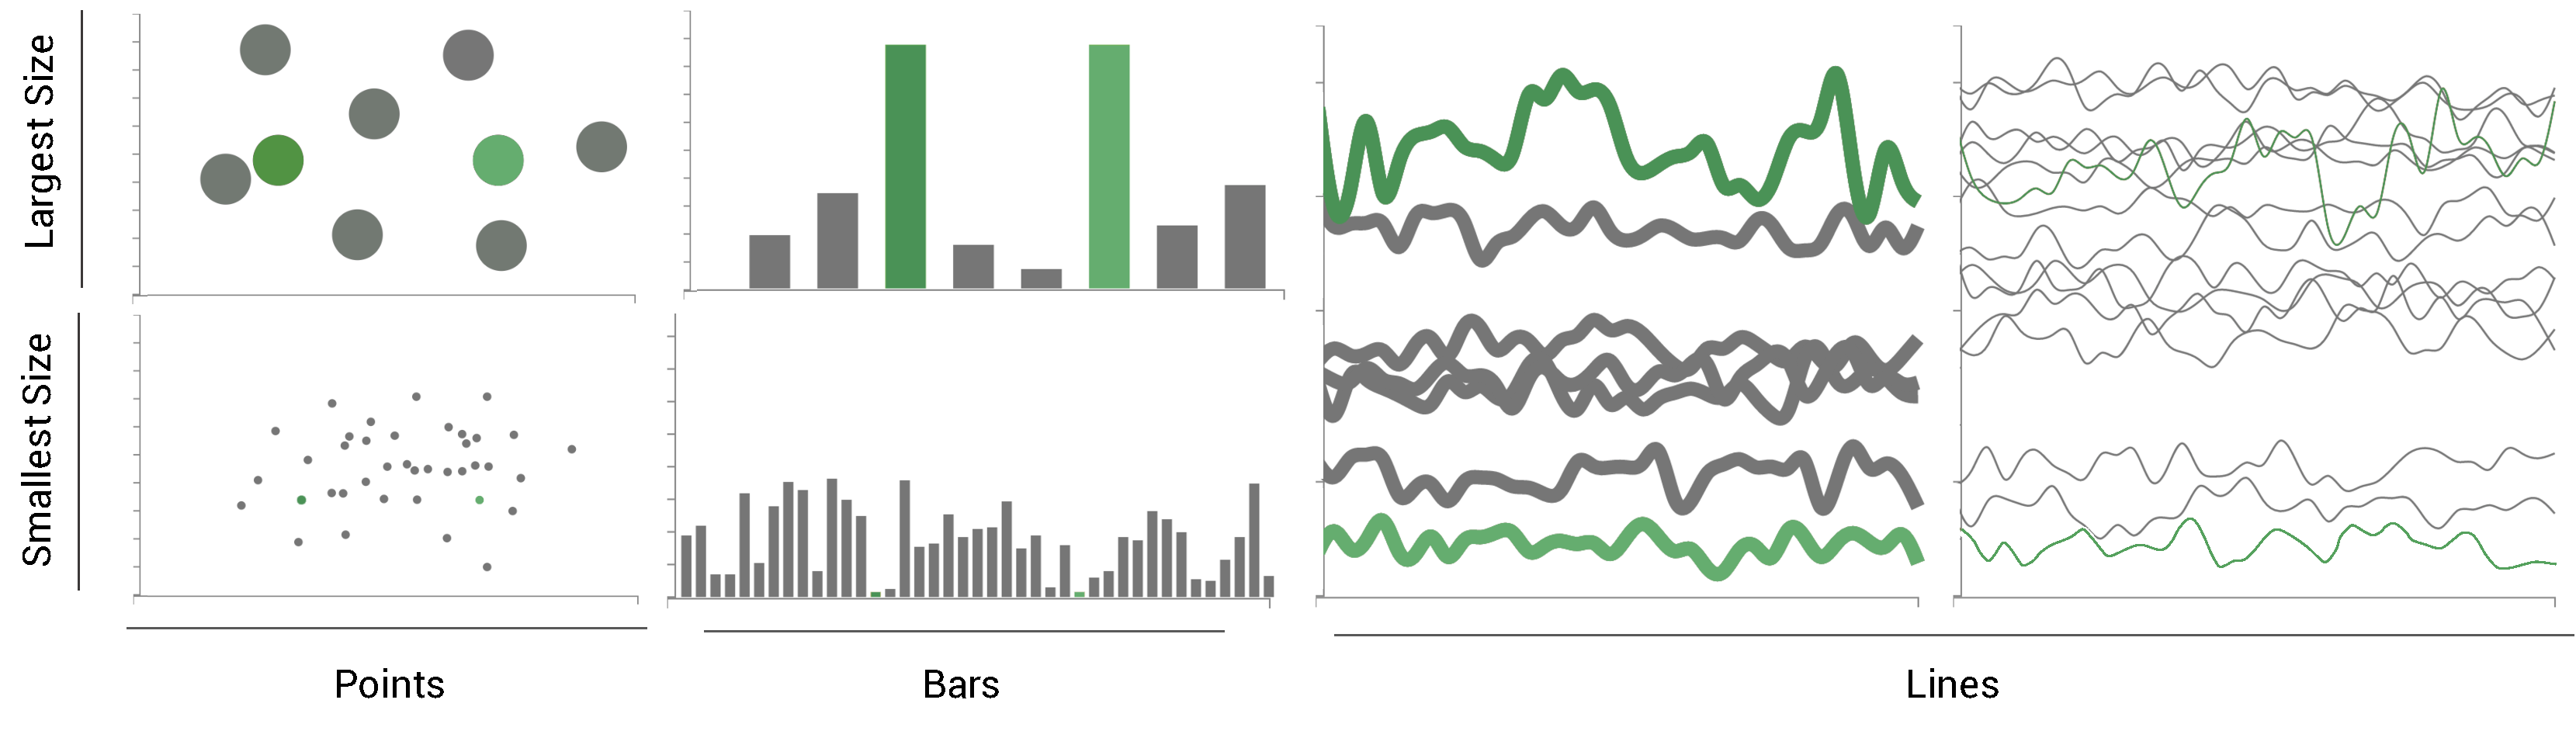
\includegraphics[width=0.48\textwidth]{teaserOne.pdf}
	\end{center}
	\caption{I build quantitative modeling of how people interpret data in different visualizations, blending vision, cognitive, and data science to encourage more effective design.}\label{color}
\end{wrapfigure}

\emph{Color Perception: } Color is commonly used to encode data; however, traditional color perception models underestimate people's abilities to distinguish colors in practice by a favor of five. This underestimation means systems using these models obfuscate differences in a significant proportion of visualized data. %I construct quantitative models of visual perception specifically tailored to visualization to correct for these issues. 
%support this research. The grant is intended to 
I received an NSF CRII (\$174,925) to 
develop computational models of color perception in visualizations and to blend these models with those capturing designer practices to construct an assistive color encoding design tool.
% blending perceptual models with statistical models of expert design practices drawn from a corpus of 
%encodings drawn from 
%designer handcrafted encodings used in existing tools. 
Unlike conventional visualization studies, this work moves beyond A/B testing to generate probabilistic models of data interpretation and design to guide effective visualizations. 
%Models developed during my Ph.D. provide significant improvements over conventional approaches, improving color disambiguation from 43\% to 99.8\% accuracy \cite{albers2014Designing}. 
This work has led to the first set of color perception models directly grounded in visualization practice
% probabilistic data-driven quantitative models that optimize conventional color spaces for archetypal visualizations, such as scatterplots and bar charts 
\cite{szafir2018Modeling} (Fig. \ref{color}). %These models provide the first set of color perception models directly grounded in visualization practice. 
These models have been integrated into leading visualization tools, including Tableau and D3, and received the Best InfoVis Paper Award at IEEE VIS, the flagship visualization conference (top paper of 170 submissions). A Ph.D. student and two M.S. students have papers in progress for submission to CHI 2019 and IEEE VIS 2019 extending these models to capture interactions between color and other encoding channels and to blend these models with Bayesian models derived from expert design recommendations to drive a novel encoding authoring system.
%to develop the underlying algorithm and tool for assistive encoding generation funded by the CRII award, 
% InfoVis Best Paper Award, selected as the top paper out of 170 submissions, and was the first solo-authored paper to receive the award in over a decade. The resulting model was adapted into the design of Tableau 10. 

\emph{Statistical Estimation: }As data continues to grow, accurate interpretation increasingly requires synthesizing 
%information across large datasets, 
statistical information such as averages and trends from large numbers of datapoints simultaneously.
% through a process known as \emph{visual aggregation}. 
However, most visualization design knowledge focuses on interpreting individual datapoints.
%As the amount of data available and the questions asked of that data continue to grow, visualizations must accommodate analyses across multiple datapoints simultaneously. However, 
%Conventional understandings of how to encode data capture comparisons between two datapoints; however, growing datasets often require analysts to synthesize information from large numbers of datapoints simultaneously, such as averages, variance, or trends. 
My research was the first to introduce ideas from \emph{ensemble coding}---people's abilities to visually estimate statistical information---to predict how visualizations might support tasks involving multiple datapoints. 
%My work has explored the idea of \emph{visual aggregation} to the creation of visualizations to remedy this knowledge gap. By integrating information about the visual system's capacity to rapidly compute statistical information about a visual scene, I modeled how the visual representations that best supported statistical tasks synthesizing information across multiple datapoints, focusing on standard aggregate statistics, such as mean and variance. 
This work demonstrated a fundamental tension between how well visualizations support comparisons at various scales: visualizations well-suited for comparing individual values perform poorly for tasks requiring people to synthesize information across multiple datapoints, while those well-suited to this synthesis perform poorly for tasks involving individual values. 
%These observations led to two novel systems: \emph{Sequence Surveyor}, a system for genetic analyses, and \emph{TextDNA}, a system for literary analysis. These systems increased the scales of data that domain experts could analyze by an order of magnitude over previous approaches. 
%I built on these findings to introduce an interdisciplinary research agenda for visualization perceptions in the era of big data.
%in the Journal of Vision. 
I extended this work by developing a framework that reveals how fundamental principles from visual perception can predict the types of statistical information people extract from different visualizations. This framework 
%introduced a new interdisciplinary research area that 
bridges computer and cognitive science and has become the fifth highest scoring Journal of Vision paper according to Altmetric (in the top 5\% of all scored publications) \cite{szafir2016Four}. This research initiated a dialog with psychologists from Northwestern University, the University of British Columbia, and MIT, lead to the founding of VisXVision, an organization of researchers aimed at encouraging collaborations between visualization and vision science. We have successfully hosted a panel at IEEE VIS and a symposium at the Vision Sciences Society Annual Meeting focusing on increasing the research dialog between these communities. Both events attracted hundreds of researchers and have led to initial collaborations between my lab and researchers at the University of Wisconsin, Carleton College, and MIT. 
%I have additionally started projects looking at visualization design and prediction in time series data and empirical data generation (led to a UROP for the student). 

%Given recent advances in automated analysis, 
\emph{Analysis Metacognition: }In order to act on data, analysts must be confident in their data and conclusions. My recent studies 
% I have extended this line of research 
%in perceptual methods 
%to 
consider how analysis tools influences cognitive aspects of data interpretation, including data credibility and classifier trust. 
%These studies focus on the role of visualization and interaction on data quality and trust. 
The first of these studies arose from 
%a collaboration with Prof. Michael Paul's group constructing a tool for iterative topic model refinement with fused 
collaborations with public health analysis 
%fusing CDC and social media data building on observations from preliminary 
fusing variable quality data sources to support mixed methods analyses \cite{pruss2018Zika}, where this fusion often generates
%. Social media data often requires analysts work with 
missing or corrupted data due to failures in data collection and alignment. An M.S. advisee (beginning her Ph.D. at Georgia Tech in Fall 2018) and I evaluated how visualization designs and statistical methods for estimating missing values influence perceived data quality, focusing on interpretation bias, confidence, credibility, reliability, and completeness \cite{song2019Wheres}. We found a systematic relationship between perceived quality and visualization structure: methods that break the visual continuity of data lead to lower perceived quality and greater interpretation bias. This study presents the most comprehensive evaluation of design methods for missing data to date and will appear at IEEE VIS 2018. 

In addition to confidence in data, trust in analysis can also encompass interpretation aided by statistical algorithms. I studied how visualizations and expert integration influence perceived trust in collaborative human-machine classification with Prof. Nisar Ahmed, a Ph.D. student, and an undergraduate (beginning his M.S. at CU in Fall 2018). We asked people to help ``train'' a classifier to distinguish between different dog breeds by asking them to confirm or adjust a predicted breed using one of eight visualizations of the classifier's prediction confidence. We presented 
%people with one of eight common visualization approaches and asked them to label images 
images using one of six policies ranging from all low-confidence images (an optimal policy for the algorithm) to all high-confidence images  (theoretically optimal for people). Our results suggest that machine-optimal policies for classifier training lead to significantly lower subjective and objective trust in outputs of a machine learning algorithm, generating a $2x$ increase in the number of times participants corrected the machine outputs. This manuscript is currently in revision for submission to CHI 2019. 

%Further, the interpretation of information doesn't stop with our sense of sight
%\todo[inline]{Cognitive Factors: Hayeong's study, Michael's study}

%\textbf{On-Going \& Future Work: }My current NSF-sponsored research integrates perceptual models with quantified models of heuristic best practices for data encoding. These heuristics describe how people select sets of colors to optimally represent data and are critical to effective visualization. However, it takes significant design expertise to use them effectively. I am creating statistical models of color encoding structure from a set of designer color maps used in visualizations to quantify these heuristics. 
%. I will model the design structure in expert-crafted encodings and blend these models with my previous perceptual models to generate a statistical model of effective color encoding. 
%integrate these models with data extracted from designer encodings to guide visualizations that adhere to both perceptual and expert designer practices. 
%I will combine the heuristic and perceptual models in an assistive design tool that allows people to rapidly construct visualizations that are grounded in perceptual science and best practices for visualizing data, reducing barriers to creating effective visualizations.

%Building on this framework, I am currently investigating the role of ensemble coding in decision making and visual data fusion. This work is measuring how visualizations can support analysts in prediction and fusion from multiple data sources across a range of domains, including defense and public health. %\vspace{-2pt}

%Interpretation of model parameters for data-driven reasoning about recommendations in QIMs

%\emph{Student Advisees: }H. Bansal, M. Iuzzolino, C. Mcguinness, R. Mustari, S. Naidu, P. Sherkane, H. Song, S. Smart, T. Umada, K. Wu\\
\emph{Funding Sources:} National Science Foundation, US Air Force\\
% (\$174,925)
\emph{Publication Venues:} IEEE VIS (Best Paper Award), Journal of Vision, Vision Sciences Society

\textbf{T2--Scalable Visualization Systems: }
%While Thread 1 allows us to understand how people interpret data in visualizations, 
Thread 2 transfers the foundational knowledge of how people interpret visualized data from T1 into systems that support effective data analysis for real-world problems. 
%My work during my Ph.D. led to systems in genomics \cite{albers2014sequence}, biochemistry \cite{sarikaya2014visualizing}, and literary analysis \cite{szafir2016textdna} that supported interactive exploration at scales an order of magnitude larger than prior approaches. 
Systems design, development, and deployment requires substantial time, especially when using the iterative user-centered design process I employ in my research. I have three systems projects currently underway with domain collaborators targeting near-term submission. These systems focus on how visualizations can support collaborative analysis between human analysts and automation in order to provide faster, more accurate, and more scalable insights into data.

\emph{Military Intelligence:} Current methods for monitoring airborne threats such as ICBMs rely on manual surveillance of satellite imagery data. This process requires substantial manpower and is highly error prone: targets are on the order of a few pixels in size. With Lockheed Martin and Prof. Nisar Ahmed under a \$353,936 grant from the US Air Force, I am investigating how visualization can improve target identification and characterization
% in military intelligence applications 
by facilitating collaboration between analysts and machine learning systems. Although machine learning enables analysts to process unprecedented quantities of data, such automation can obscure information about how data is processed and prevent analysts from applying their own contextual understandings, past experience, and domain expertise. 
%I received a e in collaboration with Prof. Nisar Ahmed (data fusion expert) and Lockheed Martin to construct 
%a system for collaborative human-in-the-loop analysis of OPIR satellite imaging data. Under this funding, we have developed 
We are developing the CAMP system (collaborative analyst-machine perception, Fig. \ref{interface}\todo{recolor and reclip}) to support intelligence analysts in identifying and characterizing potential threats in large-scale streaming satellite data by combining visualization, computer vision, and interactive machine learning. The system leverages backend data fusion algorithms from Prof. Ahmed's group with interactive visualizations developed by my lab and co-developed real-time integration of interactive analyst feedback into the classifier \cite{muesing2019}. In simulation, our approach accelerates target characterization in real-time data by 3 minutes and allows a single analyst to monitor multiple image streams simultaneously. The project has been recommended for Phase 2 funding to expand on the current research efforts and integrate CAMP into the Operational Battlespace Awareness Center. 

\begin{wrapfigure}{l}{0.5\textwidth}
	\begin{center}
		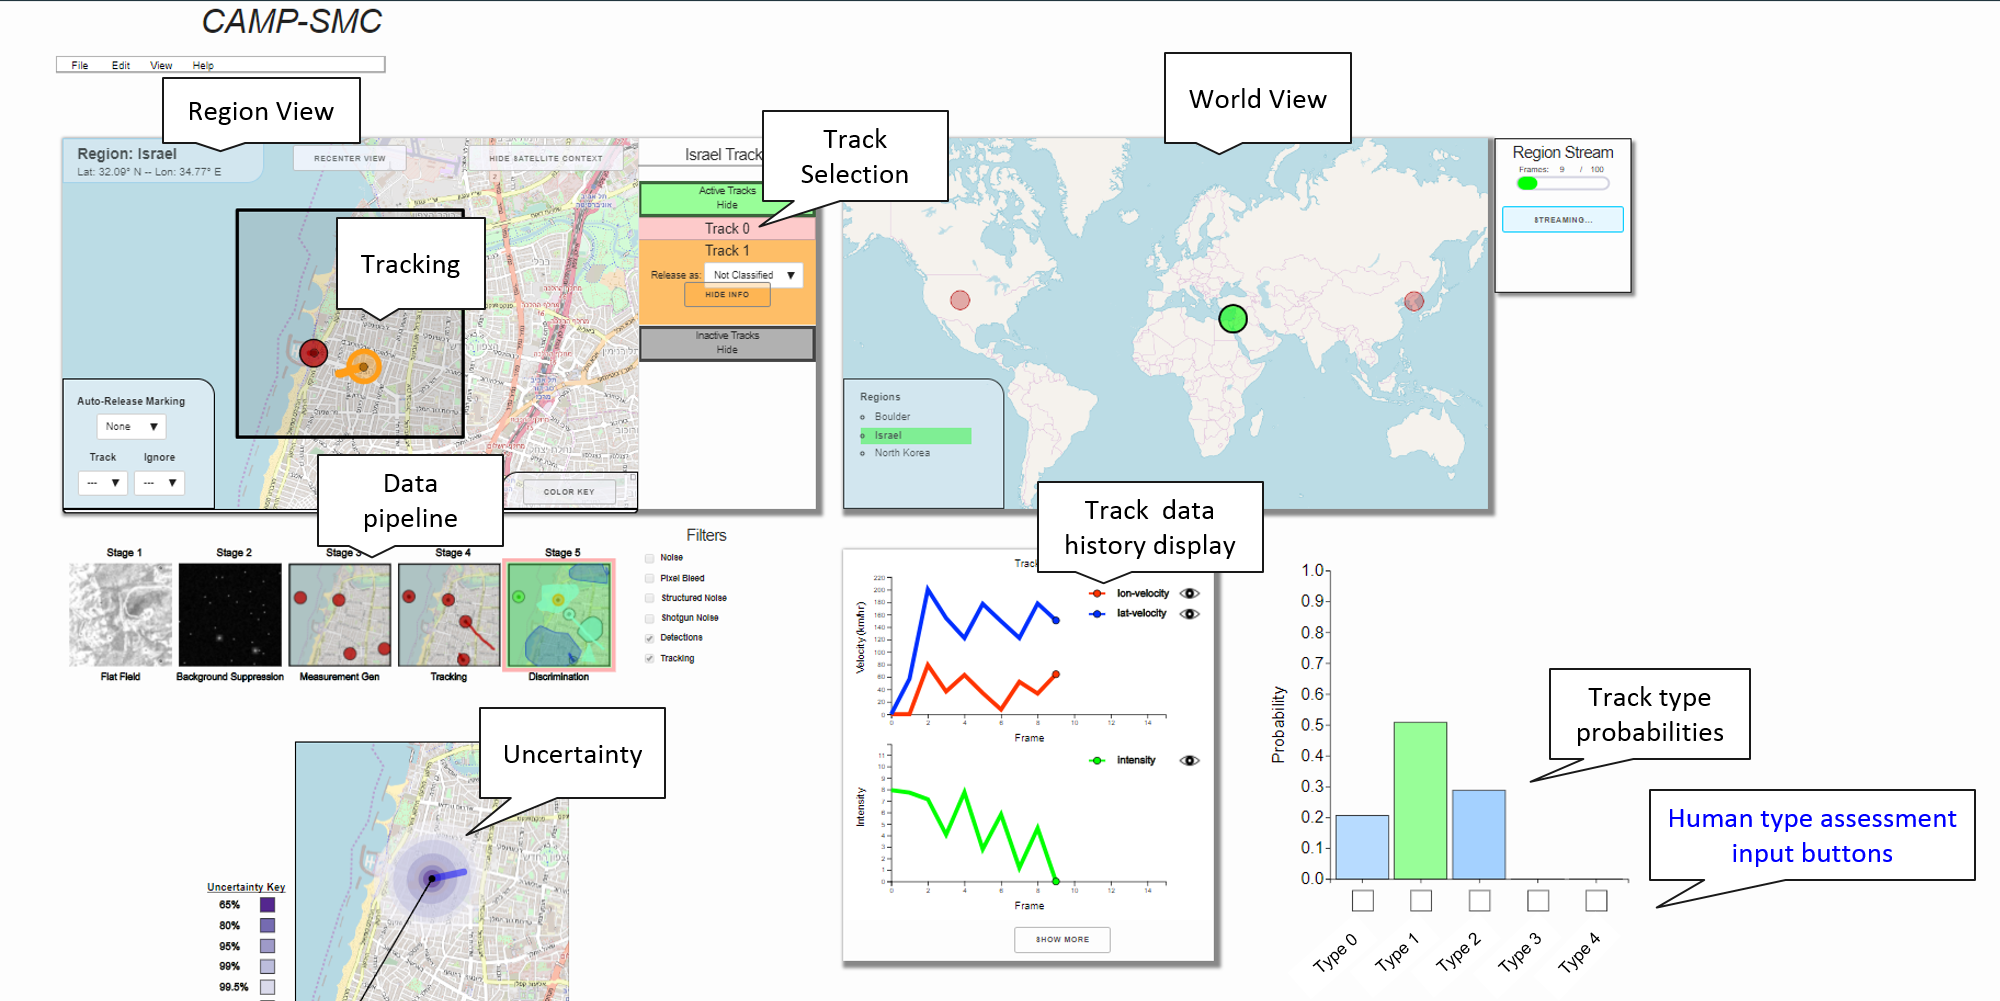
\includegraphics[width=0.48\textwidth]{interface}
	\end{center}
	\caption{The findings from T1 inform systems for collaborative human-machine analysis of large data, such as the CAMP system that enables intelligence analysts to rapidly detect and characterize threats in large-scale image data.}\label{interface}
\end{wrapfigure}

\emph{Public Health:} Public health analysts are increasingly leveraging the high-throughput data offered by social media to inform disease surveillance, information dissemination, and policy. However, social media data has low quality compared to traditional sources, such as CDC logs. In collaboration with a M.S. student, Prof. Michael Paul, and researchers at Carleton College, I am developing an interactive system fusing CDC (high quality, low throughput) and Twitter data (low quality, high throughput) to provide more holistic and scalable public health analysis enabling quality verification and contextualization for rapid disease surveillance and prediction. %Further, to provide access to the underlying information and disease dissemination, borrowing from collaborations with Prof. Paul's lab \cite{pruss2019Zika}, 
%Building on current collaborations with the Paul lab \cite{pruss2018Zika}, t
This system leverages sentiment analysis and topic modeling to extract common themes in social media data and binds these models to complementary spatiotemporal data. Analysts can refine component features and data to interactively update the automated analyses in order to mitigate quality concerns and integrate expert knowledge into decision making. The system is targeted for submission to IEEE VIS 2019.

\emph{Scaling Inductive Methods:} In collaboration with Profs. Jed Brubaker, Casey Fiesler, and Michael Paul, the third system explores how such human-in-the-loop visual analytics tools may support qualitative scholarship. Current qualitative methods require deep manual data processing, integrating context and expertise for high-quality analysis but limiting the proportion of a corpus to be analyzed and reproducibility of these analyses. These methods are applied in big data through random subsampling: the analysts only looks at a random subset of the data. This project, which has been recommended for funding by the NSF (\$1.1M), addresses this limitation by coupling machine learning, natural language processing, interactive visualization, and human-in-the-loop refinement to model qualitative text analysis in real time. As the system observes an analysts' qualitative inferences, it uses active learning to construct statistical models correlated with analyst observations. These models will scale qualitative observations to the corpus level by recommending passages correlated with different observed categories and allowing analysts full control over their workflows, access to the underlying logic behind each recommendation through in-line and corpus level visualizations, and the ability to refine recommended passages and features on-demand through interaction with these visualizations.
% and apply these models to scale an on-going QIM analysis to larger corpora by identifying potential areas of interest within a text. The algorithm observes expert analysis and steadily generates a model of different characterizations applied to text. The system will then provide recommendation of interesting passages for analysis as well as in-line visualizations of why the passage may be of interest and interactive refinement methods for dismissing and refining recommendations. The system will also allow analysts freeform exploration of label distributions and composition to 
The resulting system will allow for multiscale application of QIMs to generate classifiers that best capture expert interpretation for scalable expert-driven navigation of large corpora and analysis reproducability and explainability. 
Preliminary algorithmic development by my lab in collaboration with Prof. Brubaker's lab demonstrate that these methods can capture QIM outputs with reasonable accuracy even using basic algorithms: using a basic Na\"ive Bayes classification and traditional language features, our recommendations had an 89.9\% agreement with human experts in detecting emotional distress in unlabeled social media data.


\emph{Data Summarization:} In addition to concrete systems work, I have begun exploring how visualizations might assemble a generalizable design framework for dealing with scalability issues. In \cite{sarikayadesign}, we present a systematic qualitative survey of how visualizations summarize large datasets and patterns in these techniques for different data types, tasks, and goals. This work is co-authored by my Ph.D. advisor as the lead student author was still working under his supervision at the time. However, I served as the primary faculty supervisor and technical lead on the research. We distilled patterns in use and design in 180 systems from the visualization literature. Through this distillation, we created an initial design space to help identify current trends and open opportunities for scalable visualization designs. This paper appeared at EuroVis 2018. 

% when the amount of data far exceeds the number of available pixels. 
%While visualizations can support large-scale analyses, the number of available pixels limits the exploratory capabilities of visualization systems. Statistical analyses overcome this limitation by computationally reducing the amount of data analysts explore. However, 
%Automated data processing scales well, but hides how the reduced data was generated. This obscuration prevents analysts from applying their own understanding to the analysis problem. 
%I use visualization to enable people and machines to \emph{collaboratively} analyze data, allowing people to focus on specific patterns in the data while automation rapidly mines these patterns at scale. For example, I designed a system for computational biochemists that improved protein binding site prediction. This system paired classification algorithms with task-oriented visualizations of prediction performance, aiding analysts in rapidly identifying patterns of interest over hundreds of molecular structures
%. On-demand surface visualizations contextualized predictions and empower biochemists to 
%and interactively reparameterizing algorithms to account for prediction biases. Through a grant from the U.S. Air Force, my current research explores how visualization can enable collaborative analysis of large spatiotemporal satellite image data. I am developing a system that automatically identifies important objects and behaviors based on historical data and provides interactive mapping and metadata visualizations that describe the features and uncertainties associated with the detection. 
%Analysts interact with detailed map overlays and feature-based visualizations to provide feedback on interesting objects and behavior to the detection algorithms. 
%This research is scaffolding the development of innovative applications in drought and wildfire monitoring by facilitating seamless analysis of key anomalies in satellite imagery fused with geospatial environmental data. %\vspace{-2pt}
%\todo[inline]{OBAC Launch}

%\todo[inline]{QIMs, Public Health Analyses, Continued model-driven reasoning, Design for accessible communities}

%\emph{Student Advisees: } W. Braun, P. Deveraj, I. Fawaz, M. Iuzzolino, Y. Mahadasu, S. Nath, S. Prabhu, G. Ramkumar, H. Song, T. Umada, M. Xiao\\
\emph{Funding Sources:} National Science Foundation, US Air Force SMC-RSX\\
%National Science Foundation (\$1,070,508), US Air Force SMC-RSX (\$353,936)\\
\emph{Publication Venues:} EuroVis, AIAA@InfoTech (under review)

\textbf{T3--Embedded Analytics: }
%Building on the HCI strengths at CU has additionally allowed me to expand my research focus
Advances in mobile technologies create new opportunities for engaging context and situational awareness in data analytics tools. My third research thread explores how augmented reality (AR) might enable interactively visualizations to directly bind data representations with the physical contexts those data represent. Because research in such immersive analytics is quite nascent, my work in this area has explored contextualized AR visualization at multiple levels, ranging from perception to interaction to full system design with stakeholders in environmental science and emergency response. 

\begin{wrapfigure}{l}{0.5\textwidth}
	\begin{center}
		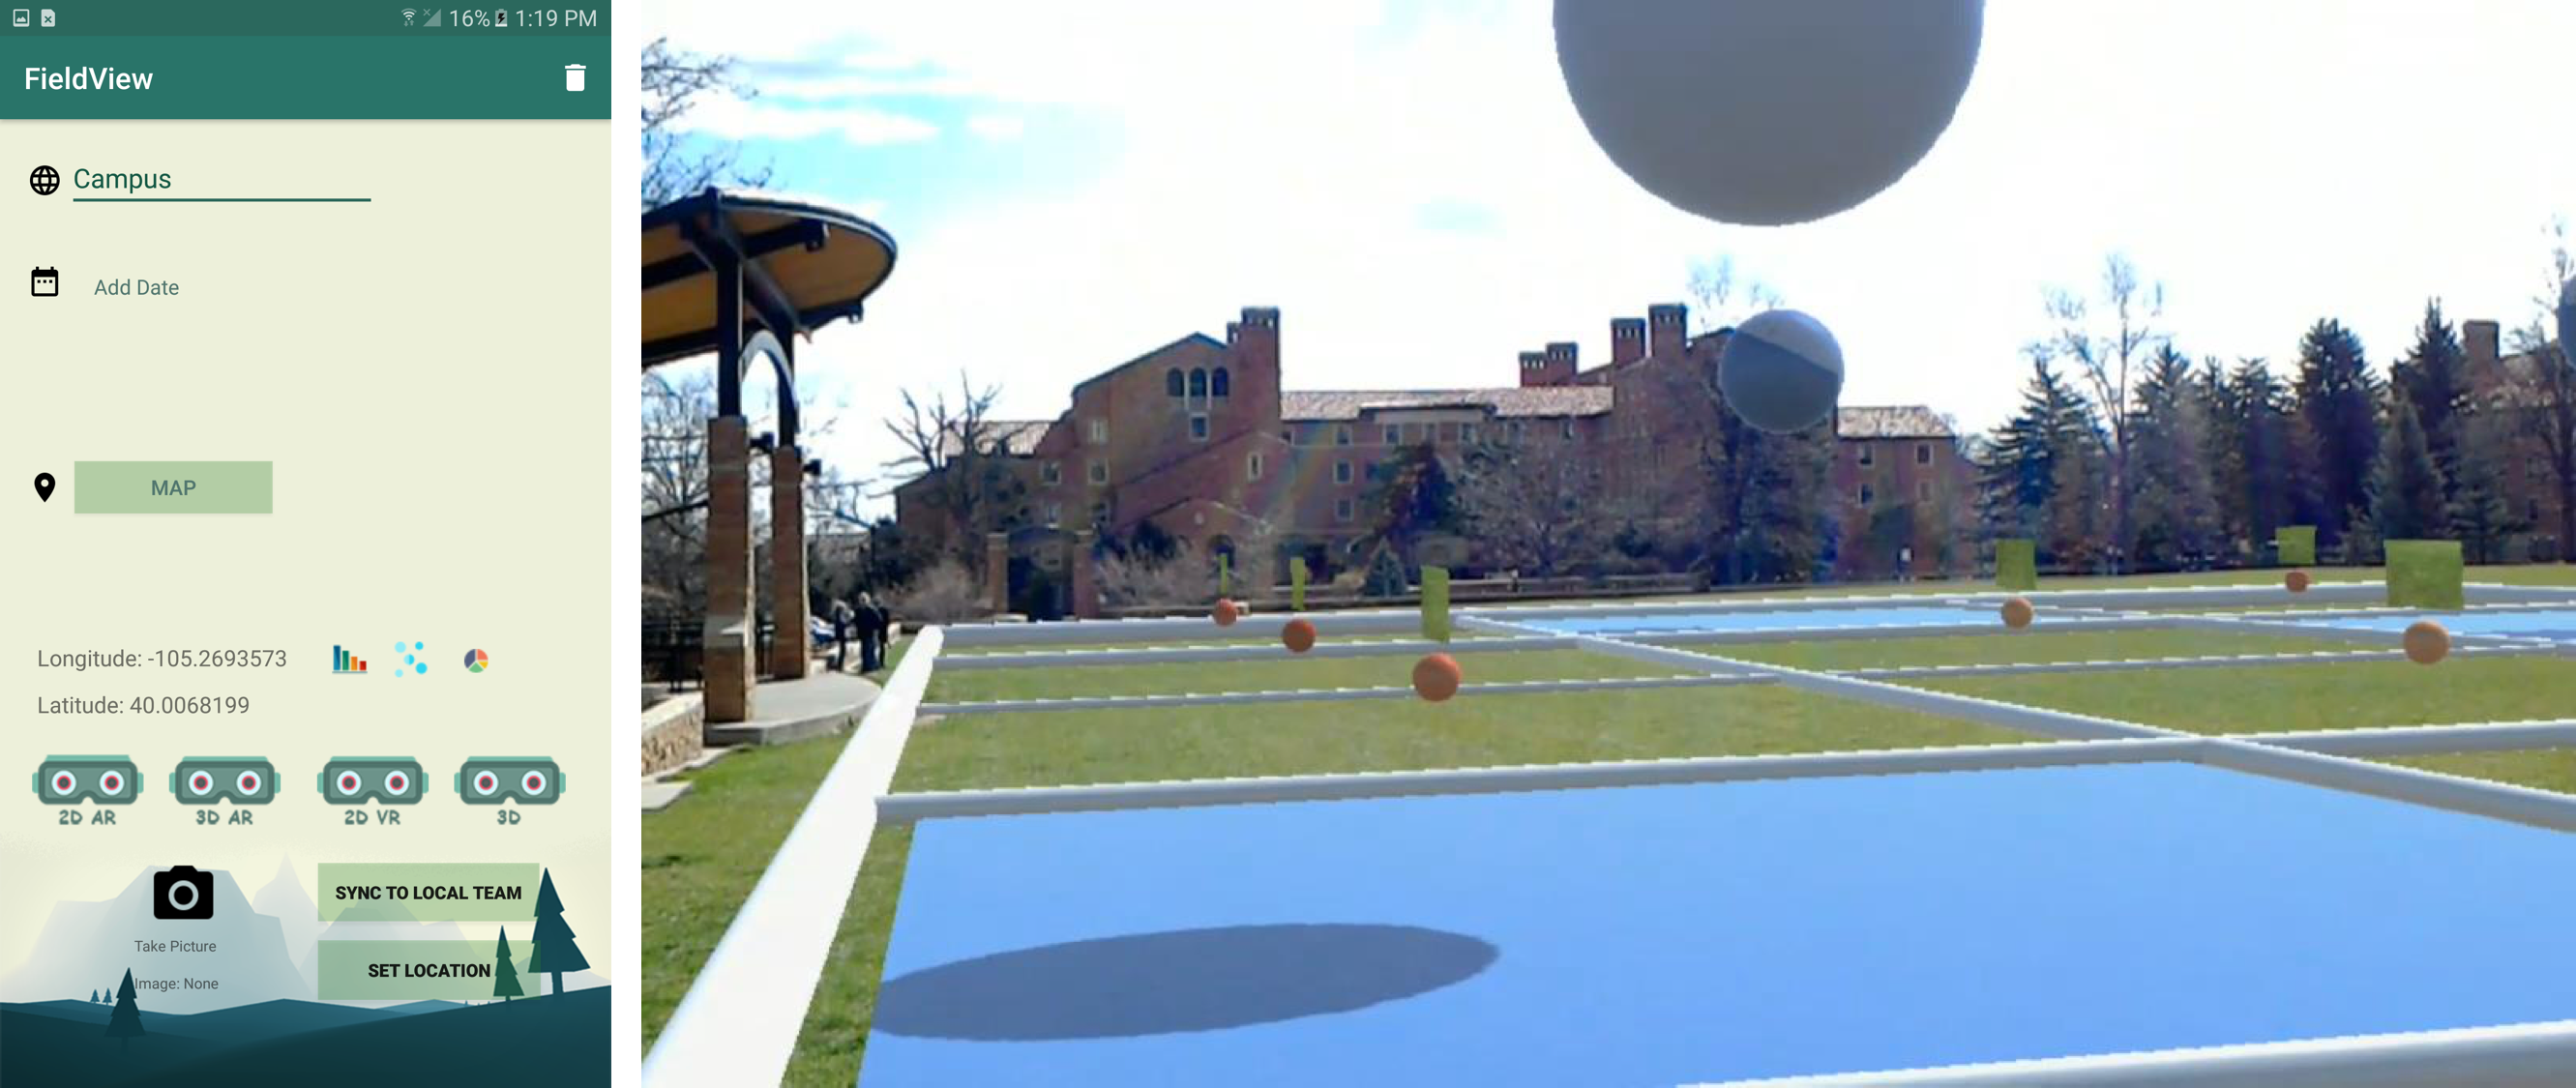
\includegraphics[width=0.48\textwidth]{fieldview}
	\end{center}
	\caption{By understanding the perceptual, cognitive, and interactive properties of immersive data analytics, we can design systems that allow analysts to capture and analyze data in real-time using mobile, cloud, and augmented reality technologies to bridge temporal and spatial gaps in field data use.}\label{fieldview}
\end{wrapfigure}

In collaboration with Prof. Dan Szafir, one M.S. student, and an undergraduate lead, we conducted a controlled laboratory study exploring how the different rendering techniques used in AR applications change where people perceive virtual objects relative to the real world \cite{diaz2017designing}. By understanding which techniques allow people to best locate virtual objects in the physical world, we can tightly bind visualized data to its corresponding physical context. In a pair of studies evaluating eight common graphics techniques conventionally correlated with spatial perceptions, we found that most conventional cues for spatial positioning had minimal effects on an object's perceived position and that synthetic stylized shadows supported more accurate and subjectively easier object localization in real-world scenes. Our results, published at ISMAR 2017,
% (the premiere conference for augmented reality research),
 suggests that computationally expensive precise rendering and artificial integration of many spatial cues (e.g., texture and lighting) are unnecessary for data localization in modern AR head-mounted displays. 
 
Embedding data in the real world may place data well beyond arm's reach, yet we know little about how to help people intuitively interact with distal data.
%. However, little is known about how to effectively engage with that data in interactive systems. 
To remedy this gap, I conducted a study in collaboration with two Ph.D. students and Profs. Shaun Kane and Jed Brubaker to empirically model preferred methods for interacting with distant data in AR \cite{whitlock2018Distal}. In this study, participants used controllers, voice, and gesture inputs to manipulate data from Internet of Things devices at 8, 12, and 16 feet. We collected objective (time to completion and task accuracy) and subjective (usability, preference, and perceived performance) data to compare the different modalities and determined that, while gesture inputs were significantly preferred overall, controller inputs performed as well or better than gesture inputs in all cases, and voice-based interactions were generally slow and cumbersome. The paper was presented at IEEE VR 2018. 

In collaboration with a Ph.D. student and two M.S. students, we used the results of these studies to design and implement an interactive system for exploring field-collected data in context. Funded by a CU Innovative Seed Grant (\$30k), we interviewed environmental scientists, field roboticists, climate scientists, and emergency responders to understand current limitations of field data analysis. These discussions identified critical gaps in time and context that limit data use, quality, collaboration, and collection practices. We used these limitations to develop a system called FieldView that uses a mobile phone application for data collection and basic visualization coupled with a cloud datastore and immersive visualization to improve in-the-field data analysis. 
%We then used this system as a design prompt to collect feedback on how the technology might enhance field data use and collection with 10 experts. \todo{check number} From these interviews, we refined 
FieldView enables situated data collection and analysis to improve data quality, context integration, and collaborative practices through situated analysis, empowering field researchers to better leverage data while in the field (Fig. \ref{fieldview}). The paper for this system is currently in revision for CHI 2019. 

With Profs. Dan Szafir and Christoffer Heckman, we had an NSF grant (\$1.2M) recommended to build a system will use FieldView's principles to improve the integration of data from both human partners and sensing devices such as robots for rapid decision making in emergency response scenarios. In this proposal, my lab will measure how the visual affordances of AR, including stereoviewing and physical context, change the effectiveness of common visualizations. We will use this data paired with interviews with emergency response teams to develop a novel visualization system for situated analysis targeted directly at emergency responders operating in the field. The goal of this system is to empower and enrich data-driven decision making in the field to improve emergency response practices under changing environments. 

%NSF Grant
%In addition to this work, I have two early-phase student-led projects exploring AR in other contexts. The first is exploring how interactive visualizations can be overlaid on physicalizations of data. The goal of this project is to leverage interactive AR to support collaborative data exploration between sighted and non-sighted users. The second project is an interactive system for in-situ prototyping. In collaboration with a Ph.D. student and an undergraduate senior capstone team, the MR-CAT system allows for situated content authoring in augmented reality, reducing barriers to environment-scale AR application development. We are currently in-process of refining the application for museum settings based on discussions with target stakeholders to support rapid prototyping of interactive AR exhibits and with Ball Aerospace for applying the prototyping solution to engineering applications including product refinement and training. 
%Justin's stuff, Ball Aerospace

%\todo[inline]{integrate images throughout}

%\emph{Student Advisees:} J. Chin, M. Natarjan, A. Thompson, M. Whitlock, K. Wu, MR-CAT Team\\
\emph{Funding Sources:} National Science Foundation, CU Innovative Seed Grant Program\\
%National Science Foundation (\$1,194,056), Innovative Seed Grant Program (\$30,000)  \\
\emph{Publication Venues:} IEEE VR, ACM/IEEE ISMAR

\section*{Career Research Trajectory}

My overall research agenda aims to 
%understand how we can leverage visualization to 
make exploratory data analysis more accurate, scalable, and holistic through visualization. I achieve this by modeling how people interpret visualizations, using this understanding to drive novel analytic systems, and integrating novel technologies into visualization approaches in order to overcome contextual barriers to analysis. My work at CU has resulted in seven top-tier conference and journal publications, over \$2M in funding from national agencies, and research mentorship of 23 students. 

Through the on-going and up-coming projects listed above, my near-term research agenda will focus more deeply on system development. Recent funding successes afford the opportunity to shift more time from grants to active research and expanded collaboration with researchers external to CU.
% with which discussions have already begun for preliminary steps towards publishable interdisciplinary projects. 
To support this work, I intend to focus additional efforts towards recruiting additional Ph.D. students through funded RAships in Information Science.  
%Future trajectory: Focus more on system development, slowing grant writing and focusing on production in the near term. 
%Target Impact: make data science more accessible through empirical, user-centered approaches. Benefits both designers and users
My goal 
%through this research 
is to advance 
%the field of data science 
data science by developing tools, guidelines, models, and methods that empower people, allowing them to drive analyses through interactive systems that support reliable and meaningful use of data.
%In my research and my work as founding faculty in the new Department of Information Science at CU Boulder, I aim to advance the field of data science by developing tools and methods that empower people, allowing them to drive analyses through interactive systems that support reliable and meaningful use of data. 


{
\vspace{4pt}
\noindent
\textbf{References}
\vspace{-24pt}
\renewcommand\refname{\vskip -1cm}
\small
\bibliographystyle{abbrv}
\bibliography{main}
}


\pagebreak
\setcounter{page}{1}


\end{document}
